% !TEX root = ../../main.tex

\subsection{A study on a novel MOF}

With the methods of characterisation through calorimetry
outlined on a reference material, a similar study on a 
MOF sample can be performed. The aim is to screen for 
potentially interesting features for use in gas 
storage and separation.

\subsubsection{Material}

Zr Fumarate, also known as MOF-801, is a fumaric 
acid analogue of the well-known UiO-66(Zr) 
framework~\cite{wissmannModulatedSynthesisZrfumarate2012}.
Its structure is similar to that of UiO-66, although 
the smaller non-linear linker leads to a lowering of 
symmetry and a slight tilting in the Zr-O clusters,
as depicted in \autoref{calo:fgr:zrfum-structure}.
The MOF is synthesised using the modulated synthesis method and 
formic acid as the modulator to increase the crystalinity of the
material. Indeed, when not using this approach, the resulting
material is nearly amorphous~\cite{zahnInsightMechanismModulated2014}.
In this study the sample was synthesised according to the procedure 
detailed in \autoref{appx:synthesis:zrformate}.

\begin{figure}[htb]
    \centering
    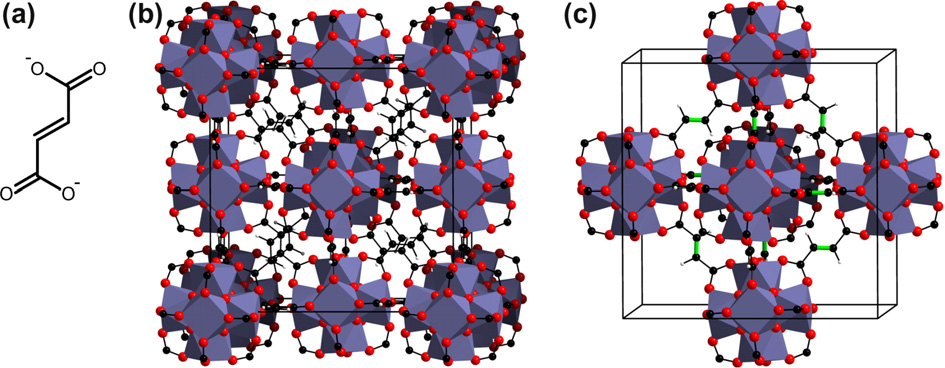
\includegraphics[width=0.8\textwidth]{zrfum/structure}%
    \caption{(a) The fumarate linker used in the Zr Fumarate
    MOF, an ionic form of \textit{trans}-butenedioic acid and
    (b) and (c) the structural model of the MOF. Illustration
    adapted from~\citeauthor{wissmannModulatedSynthesisZrfumarate2012}%
    \cite{wissmannModulatedSynthesisZrfumarate2012}.}%
    \label{calo:fgr:zrfum-structure}
\end{figure}

Zr Fumarate has recently been the subject of interest due to its
high water stability~\cite{zahnWaterbornZrbasedPorous2015}, 
as well as its potential to be synthesised through green synthesis
routes~\cite{reinschFacileGreenRoute2016} or direct
monolith formation with a gel approach~\cite{buekenGelbasedMorphologicalDesign2017}.

Furthermore, the material has a remarkably steep water adsorption
behaviour at low pressure~\cite{furukawaWaterAdsorptionPorous2014},
which has led to its possible application as a water scavenger 
membrane~\cite{baeTransparentMetalOrganic2016} or in a water 
harvesting device which would capture water from air in low relative
humidity environments such as the desert. While initial 
attempts~\cite{kimWaterHarvestingAir2017} were criticised for
overpromising performance, more recent modifications to such 
a system have addressed some of these 
concerns~\cite{kimAdsorptionbasedAtmosphericWater2018}.

The low relative pressure of water adsorption has highlighted
the contribution of defects~\cite{choiRoleStructuralDefects2018} in 
shifting the adsorption isotherm, an effect arising from cooperative
interactions and initial clustering of water molecules on defect
sites~\cite{vandichelWaterCoordinationDehydration2016}.

As the properties of the MOF diverge from the ideal properties
indicated by the structure, an experimental study to test for the adsorption
or separation of other molecules may reveal unexpected 
applications.

\subsubsection{Results}

Adsorption isotherms of nine probe gasses were recorded at 
\SI{303}{\kelvin} through combined manometry and microcalorimetry
as described in \autoref{calo:method:calo}. The complete 
dataset can be seen in \autoref{calo:fgr:zrfum-data}.
The results are remarkably similar to the Takeda 5A carbon, with 
very similar trends visible. All isotherms are somewhat 
shifted downwards, which suggest less interaction with the 
pore walls and a lower total pore volume. The enthalpies of 
adsorption are on average lower by \SIrange{5}{7}{\kilo\joule\per\mol},
confirming that the guest-host attraction is overall lower than
in the carbon. Argon, oxygen and nitrogen isotherms are essentially
following Henry's law in the measured pressure range, with nearly constant
enthalpies of adsorption. Carbon dioxide adsorption enthalpy is seen to take
place on specific sites at the start of the isotherm, then
decreasing until around \SI{25}{{\kilo\joule\per\mol}}. Cooperative
interactions take over afterwards, slowly increasing the enthalpy 
of adsorption.

\begin{figure}[htb]
    \centering

	\begin{subfigure}[b]{.45\textwidth}
        \centering
        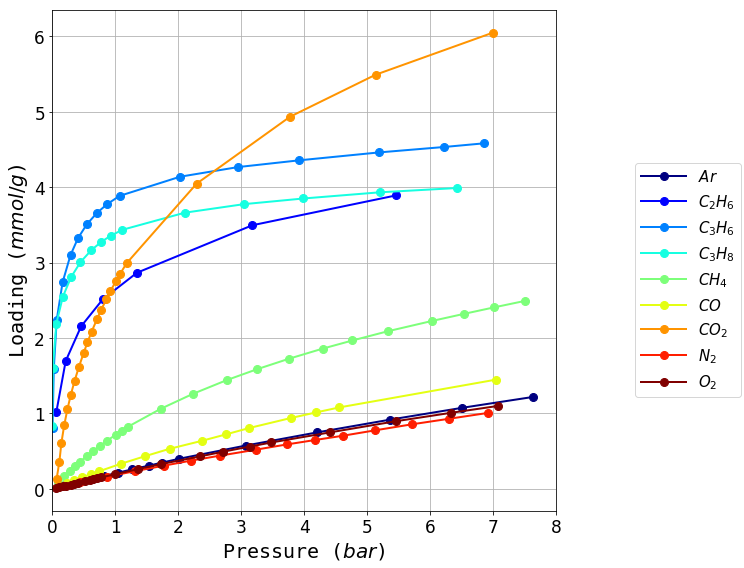
\includegraphics[width=\linewidth]{zrfum/zrfum-dataset}
        \caption{}%
        \label{calo:fgr:zrfum-dataset}
    \end{subfigure}%
	\quad
	\begin{subfigure}[b]{.45\textwidth}
        \centering
        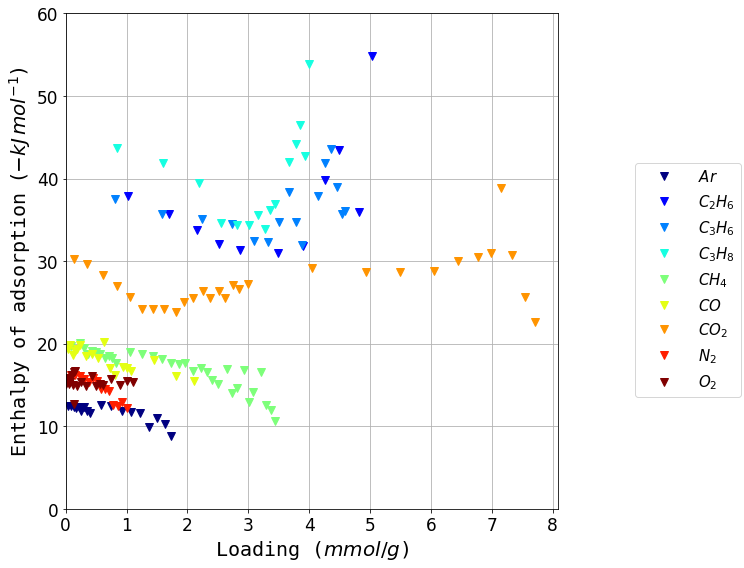
\includegraphics[width=\linewidth]{zrfum/zrfum-enthalpy}
        \caption{}%
        \label{calo:fgr:zrfum-enthalpy}
    \end{subfigure}
    \caption{(a) The experimental isotherms of all recorded gases and
    (b) the corresponding enthalpy curves.}%
    \label{calo:fgr:zrfum-data}

\end{figure}

The propane and propylene isotherms also show a higher total
loading for propylene at the plateau. However, the enthalpy
curve suggest a higher adsorption enthalpy of propane at lower
loading. A similar plot for initial Henry's constant and
enthalpy of adsorption at zero loading, in \autoref{calo:fgr:zrfum-trends},
confirms this trend, with propylene showing a decreased value
in both parameters. As propane still lies on the trendline generated
by unsaturated hydrocarbons, it does not seem that it possesses any
increased specific interactions with the MOF surface. Instead, 
the expected values for propylene are lower than those of its
saturated counterpart. It should be pointed out that the
slope of the trendline is lower than that of the Takeda 5A. This slope 
can be thought of as a measure of the non-specific interaction strength
of the adsorbate surface.

\begin{figure}[htb]
    \centering
    
    \begin{subfigure}[b]{0.5\textwidth}
        \centering
        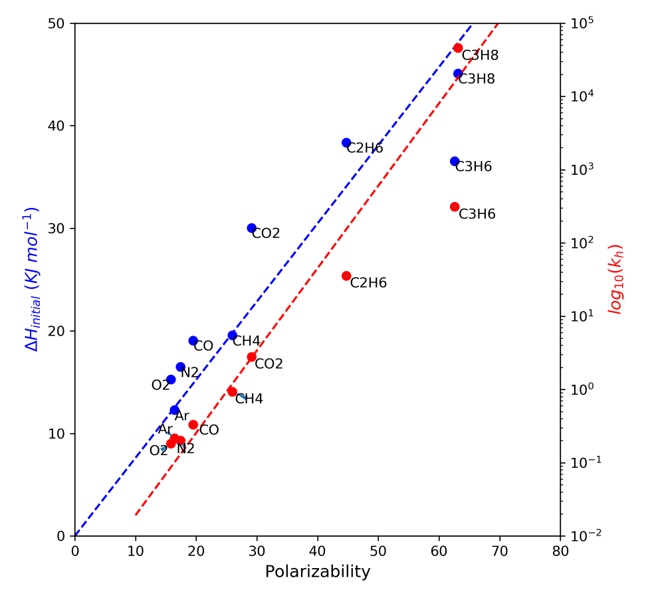
\includegraphics[width=\linewidth]{zrfum/zrfum-enth-henry}
        \caption{}%
        \label{calo:fgr:zrfum-trends}
    \end{subfigure}%
    \begin{subfigure}[b]{0.45\textwidth}
        \centering
        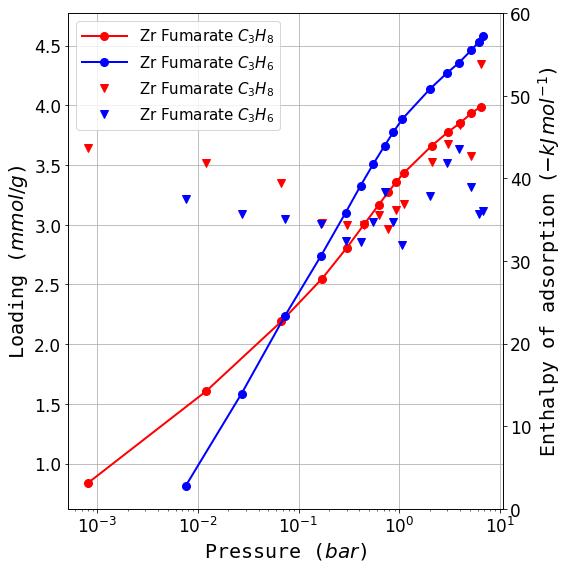
\includegraphics[width=\linewidth]{zrfum/zrfum-close}
        \caption{}%
        \label{calo:fgr:zrfum-close}
    \end{subfigure}%
    \caption{(a) Calculated trends for initial heat of adsorption (red) and 
    Henry's constant (blue) as a function of polarizability for 
    Zr Fumarate. The dotted lines are best fit lines to 
    the series of unsaturated hydrocarbons. (b) Logarithmic form of the 
    propane and propylene isotherms.}%
    \label{calo:fgr:zrfum-analysis}

\end{figure}

When examining the low pressure region of the two isotherms 
(\autoref{calo:fgr:zrfum-close}) a preference for propane over
propylene can be observed, which is the source of the anomaly
in the polarizability graph. The isotherms then ``cross over'' 
at higher pressures.
This behaviour has been reproduced in when measuring the same 
isotherms with a commercial apparatus.
A higher selectivity for propylene adsorption is not uncommon
in materials with open metal sites which can interact with 
the \(\pi\) electrons of the 
molecule~\cite{rubesAdsorptionPropanePropylene2013}.
Furthermore, MOFs with pore sizes perfectly tuned for kinetically
selective adsorption of propylene over propane have been shown 
to exist~\cite{leeKineticSeparationPropene2011}. However,
the preference for propane in this material is surprising.
The effect itself is unlikely to arise from simple diffusion
effects of~\cite{granatoDiffusionPropanePropylene2010}, although
it has been shown~\cite{combarizaPropanePropyleneDiffusion2009}
that pore windows can dominate diffusion behaviour. A contribution
from framework defects is also be likely, as the 
crystal structure calculated pore volume is 40\% of the total
volume as determined from the propane adsorption isotherm.

\begin{figure}[htb]
    \centering
    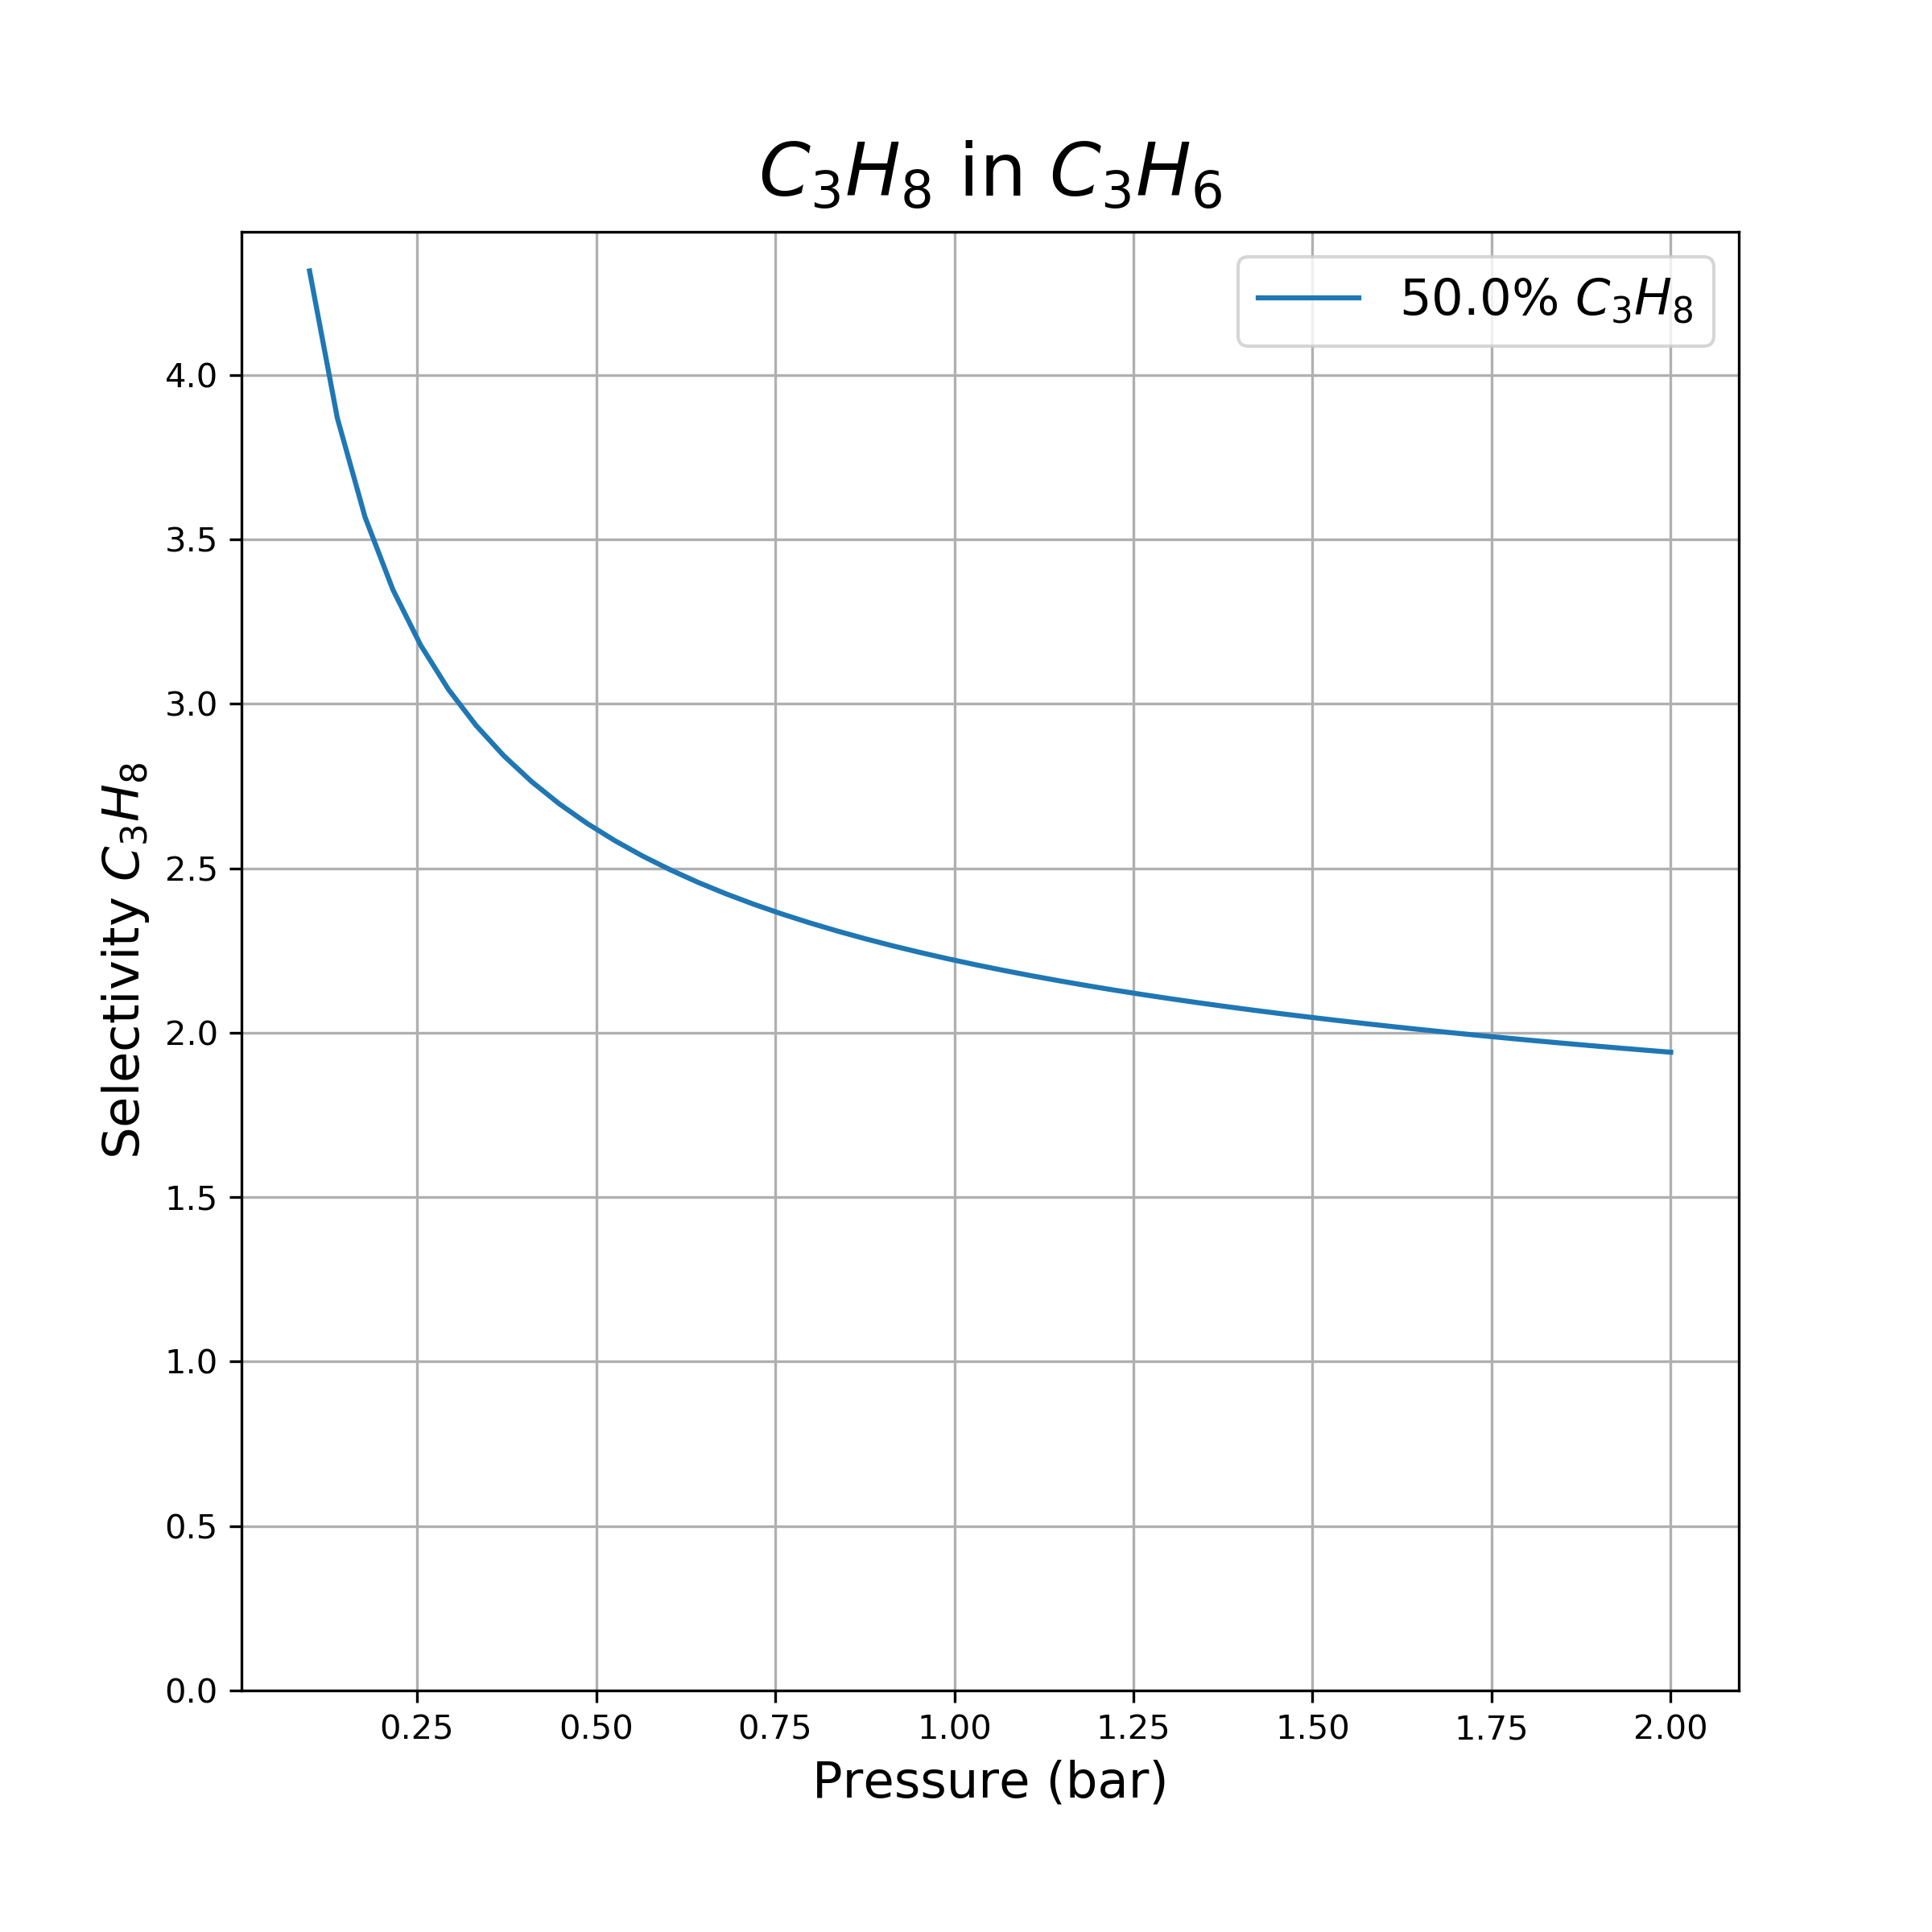
\includegraphics[width=0.5\linewidth]{zrfum/zrfum-iast}
    \caption{IAST simulation of an equimolar mixture of 
    propane and propylene on Zr Fumarate}%
    \label{calo:fgr:zrfum-iast}

\end{figure}

To observe the impact on separation efficiency, the two isotherms 
are fitted with the best conforming model, in this case
double site Langmuir, and IAST simulations of an equimolar mixture
of propane and propylene are carried out as seen in 
\autoref{calo:fgr:zrfum-iast}. A selectivity of 4--2 for 
propane is predicted by IAST, which may be of interest in 
large-scale processes, as even a small separation factor 
improvement may yield large energy savings.

\todo{should i put water isotherms, tga or any other data?}